\chapter{Resultados}

Neste capítulo serão apresentados os resultados obtidos nos testes de carga e busca dos dados. Os testes foram realizados em quatro configurações de \emph{cluster}, com uma, duas, quatro e seis máquinas, a fim de se analisar a melhora do desempenho de um banco de dados não relacional ao se aumentar o número de nós. Além disso, em cada configuração de \emph{cluster}, foram realizados três testes com diferentes volumes de dados. 

Em cada configuração de teste foram realizadas dez repetições, tanto na inserção quanto na busca, a fim de garantir resultados mais consistentes. 

\section{Carga de dados}
A carga de dados foi relizada a partir da leitura dos arquivos \emph{.csv} de dados do Bolsa Família, com seleção das colunas a serem utilizadas e tratamento de alguns campos.
Os dados foram carregados a partir de uma única máquina utilizando aplicação desenvolvida. Foi feita também uma comparação entre os tempos observados em cada uma das configurações utilizadas. Esta seção descreve em detalhes essas operações.

\subsection{Preparação e carga}
Foi desenvolvida uma aplicação Java responsável por toda a operação da inserção dos dados com uso do \emph{driver} da \emph{Datastax}. Essa inserção é realizada selecionando-se os campos a serem inseridos e tratando alguns campos com formatos não suportados pelo Cassandra. 

Foi necessário a remoção do separador de milhares(','), além da formatação do período do benefício, que originalmente segue o padrão MM/AAAA, que não é suportado pelo Cassandra. Essa data teve que ser alterada, adicionando-se o o primeiro dia de cada mês ao formato original.

A carga foi realizada com três volumes de dados, equivalentes a seis meses, um ano e dois anos de dados. A tabela~\ref{tab:volume} apresenta o volume total dos dados inseridos em cada uma dessas cargas.

\begin{table}[]
	\centering
	\caption{Volume da dados}
	\label{tab:volume}
	\begin{tabular}{ll}
		\textbf{Carga} & \textbf{Tamanho} \\ \hline
		6 meses        &  2,94 GB             \\ \hline
		1 ano          &  5,88 GB             \\ \hline
		2 anos         &  11,79 GB             \\ \hline
	\end{tabular}
\end{table}

A inserção foi realizada utilizando funções padrões do driver da Datastax, com uso da linguagem CQL com uma \emph{query} simples de inserção e preenchimento dos parâmetros ~\ref{lst:clq_insert}. As operações foram realizadas com seis \emph{threads} simultâneas, valor que apresentou o melhor resultado nos testes. 

\begin{lstlisting}[caption={Código CQL para inserção},label={lst:clq_insert},language=SQL]
INSERT INTO bolsa_familia.dados (uf, cod_municipio, nome_municipio, nis_favorecido, nome_favorecido, fonte, valor, periodo) VALUES (?, ?, ?, ?, ?, ?, ?, ?)
\end{lstlisting}

A Tabela~\ref{tb_insert} apresenta os tempos obtidos na inserção dos dados nos diferentes ambientes e volumes de dados. O gráfico~\ref{fig:graphinsert} apresenta os mesmo dados para melhor visualização.


\begin{table}[]
	\centering
	\caption{Inserção}
	\label{tb_insert}
	\begin{tabular}{lllll}
		\textbf{Tamanho}	& \textbf{1 nó} & \textbf{2 nós} & \textbf{4 nós} & \textbf{6 nós} \\ \hline
		\textbf{6 meses}    & 25m37s        & 28m02s         & 27m15s         & 26m29s         \\ \hline
		\textbf{1 ano}      & 51m19s        & 55m25s         & 54m16s         & 52m22s         \\ \hline
		\textbf{2 anos}     & 01h44m53s     & 01h59m17s      & 01h46m57s      & 01h43m56s      \\ \hline
	\end{tabular}
\end{table}

\subsection{Comparação dos ambientes}

Pelos resultados obtidos é possível observar uma melhora no tempo de inserção com uso de mais máquinas no \emph{cluster}, com exceção do caso de apenas um nó, devido às limitações da rede na comunicação entre as máquinas. Mesmo assim, é possível observar que ao se aumentar o volume dos dados, um aumento do número de máquinas apresenta uma tendência de melhora nos tempos obtidos.

Para o teste com dados de 6 meses, a melhoria média ao se aumentar o número de máquinas foi de \textbf{2,8\%}, para 1 ano foi de \textbf{2,78\%}, e para 2 anos foi de \textbf{6,58\%}, desconsiderando-se os resultados com uma máquina.

\begin{figure}[!htb]
	\centering
	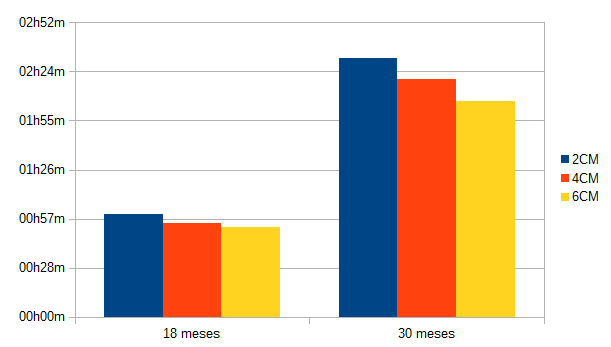
\includegraphics[width=1\textwidth]{figuras/graphinsert.png}
	\caption{Inserção de dados}
	\label{fig:graphinsert}
\end{figure}

%\section{Extração de dados}
%Assim como na carga de dados, para os testes de extração foram utilizados quatro configurações de cluster, com três diferentes volumes de dados. Foram realizadas consultas de agregação de dados e buscas por registros específicos.
%As consultas por agregação estão listadas na tabela~\ref{tab:consultasagregacao}, enquanto os registros buscados estão listados na tabela~\ref{tab:consultasbuscas}.
%
%As tabelas~\ref{tab:select_agreg} e ~\ref{tab:select_busca} apresenta os tempos obtidos na extração agregada e de busca de dados nos diferentes ambientes e volumes de dados.
%
%\begin{table}[]
%	\centering
%	\caption{Agregação de dados}
%	\label{tab:select_agreg}
%	\begin{tabular}{lllll}
%		\textbf{Tamanho} & \textbf{1 nó} & \textbf{2 nós} & \textbf{4 nós} & \textbf{6 nós} \\ \hline
%		6 meses          & 01m04s        & 01m43s         & 02m39s         & 03m01s         \\ \hline
%		1 ano            & 02m01s        & 03m13s         & 05m00s         & 09m29s         \\ \hline
%		2 anos           & 04m02s        & 11m22s         & 11m13s         & 09m29s         \\ \hline
%	\end{tabular}
%\end{table}
%
%\begin{table}[]
%	\centering
%	\caption{Busca de dados}
%	\label{tab:select_busca}
%	\begin{tabular}{lllll}
%		\textbf{Tamanho} & \textbf{1 nó} & \textbf{2 nós} & \textbf{4 nós} & \textbf{6 nós} \\ \hline
%		6 meses          & 0,0112s       & 0,0188s        & 0,0326s        & 0,0376s        \\ \hline
%		1 ano            & 0,0844s       & 0,0399s        & 0,0463s        & 0,0579s        \\ \hline
%		2 anos           & 0,2253s       & 0,2492s        & 0,1121s        & 0,0579s        \\ \hline
%	\end{tabular}
%\end{table}
%
%\subsection{Comparação do ambiente}